\makeatletter
\def\input@path{{../../}}
\makeatother
\documentclass[../../main.tex]{subfiles}

\graphicspath{
	{../../img/}
	{../img/}
	{img/}
}

\begin{document}
	
	
	\subsection{Вычисление объемов с помощью ПовИ}
	Поскольку объем $W$ может быть найден по формуле
	\[ V = \iiint \limits_W dx dy dz, \]
	то, если в формуле Гаусса-Остроградского подынтегральная функция тождественно 
	равна $1$, то имеем
	\[ V = \iint \limits_{\pi} Pdydz+Qdxdz+Rdxdy = * \]
	
	Это будет выполняться, например, для
	\[ *=  \iint \limits_{\pi} x \, dydz = \iint \limits_{\pi} y \, dxdz = \iint 
	\limits_{\pi} z \, dxdy = \iint \limits_{\pi}  \frac{1}{3} x \, dydz + 
	\frac{1}{3} y \, dxdz + \frac{1}{3} z \, dxdy. \]
	
	\begin{example}
	
	Найти объем тела, ограниченного поверхностью, которая задается формулой:
	
	\[ \pi:\begin{cases} x=\left( b + a \cos{v} \right) \cos{u}, \\ 
	y = \left( b + a \cos{v} \right) \sin{u}, \\ 
	z= a \sin{v},
	\end{cases} \]
	где
	$- \pi \leq v \leq \pi$,\,\
	$0 \leq u \leq 2\pi$,\,\
	$0 < a < b$.
	
	Если окружность в точке $(b,0)$ с радиусом $a$ вращать вокруг оси $Oz$, 
	получим тело вращения. Это тело представляет собой тор.
	\begin{center}
		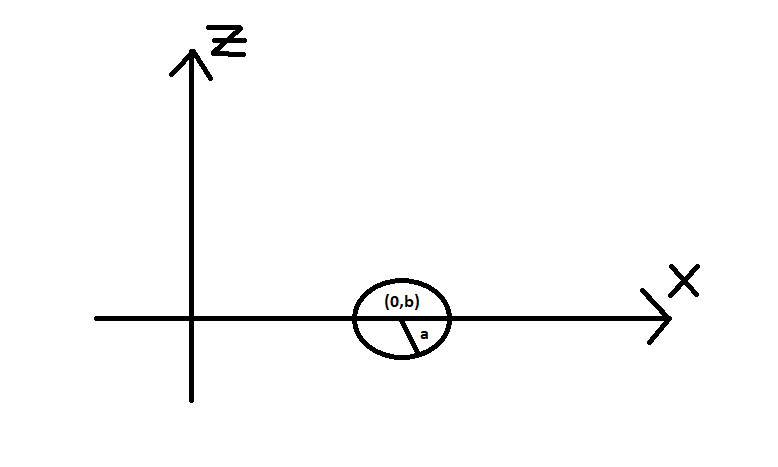
\includegraphics[scale = 0.8]{lec_25_Thor_POVI}
	\end{center}
	
	Воспользуемся формулой:
	
	\[ V = \iint \limits_{\pi} zdxdy = \int_{0}^{2\pi}du \int_{-\pi}^{\pi}z\left( 
	u,v \right) \cdot C \, dudv, \] 
	где
	\[ C = \begin{vmatrix}
	x_u' & y_u' \\
	x_v' & y_v' \\
	\end{vmatrix} = x_u'  y_v' - x_v'  y_u' = a \sin^2{u} \sin{v} \left( b + 
	a\cos{v} \right) + a \cos^2{u} \sin{v} \left( b + a\cos{v} \right)  = a 
	\left( b + a\cos{v} \right) \sin{v}. \]
	Тогда
	\begin{gather*} V = a^2 \int\limits_{0}^{2\pi} du \int\limits_{-\pi}^{\pi} 
	\sin^2{v} \left( b + a\cos{v} \right) \, dv = 2\pi a^2 \left(  a 
	\int\limits_{-\pi}^{\pi } \sin^2{v} \cos{v} \, dv + b \int\limits_{-\pi}^{\pi 
	} \frac{1-\cos{2v}}{2} \, dv  \right) = \\ = 2\pi a^2 (0 + b\cdot(\pi+0))  = 
	2\pi^2a^2b = \pi a^2\cdot 2\pi b. \end{gather*}
	\end{example}

	\section{Формула Стокса}
	
	Пусть есть поверхность $\pi$, ограниченная кривой $l$. Говорят, что 
	направление обхода границы $l$ \emph{согласовано} с выбором поверхности 
	$\pi$, если при движении в таком направлении поверхность $\pi$ остается 
	слева, а вектор нормали к поверхности $\pi$ направлен снизу вверх по 
	отношению к наблюдателю.
	
	\begin{center}
		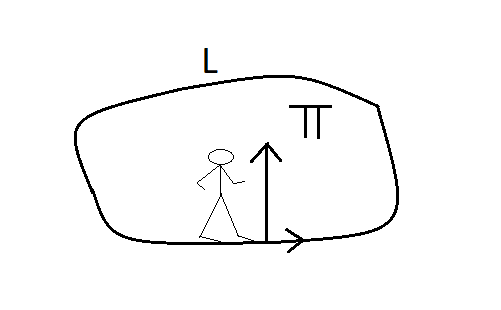
\includegraphics[scale = 0.8]{lec_25_Human_direction}
	\end{center}
	
	Будем предполагать, что в дальнейшем такое согласование имеет место.
	
	\begin{thm}[формула Стокса]
		Пусть функции $P,Q,R$ непрерывны и имеют непрерывные частные производные 
		первого порядка в области $D$. Тогда справедлива формула
		\[\boxed{ \oint \limits_L P \, dx + Q \, dy + R \, dz = \iint \limits_{\pi} 
		\left( Q_x' - P_y'\right)dxdy + \left( R_y' - Q_z'\right)dydz + \left( P_z' 
		- R_x'\right)dzdx. }\]
	\end{thm}
	
		Как ее запомнить?
		
		\begin{center}
			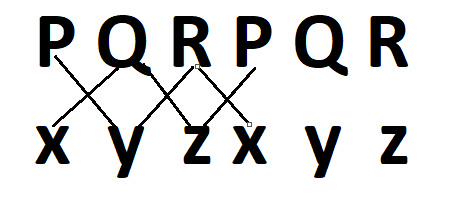
\includegraphics[scale = 0.6]{lec_25_PQR}
		\end{center}
		
		\begin{proof}
			Пусть $\pi$ задана уравнениями:
			
			\[ \pi : \begin{cases} 
			x = x\left( u,v\right), \\ 
			y = u\left( u,v\right), \\ 
			z = z\left( u,v\right),  
			\end{cases} \]
			где $\left( u,v \right) \in \Delta \subset \R^2$ и $\lambda$~--- 
			граница области $\Delta$:
			\[ \lambda : \begin{cases} 
			u = u \left( t \right),  \\ 
			v = v \left( t \right), \\ 
			t \in T \subset \R.  
			\end{cases} \]
			
			Совершенно понятно, что если мы возьмем точки на границе $\lambda$, то 
			получим точки на области $\pi$. Возьмем произвольное $t$, тогда для точки
			 \begin{gather*} x = x( u( t), v( t)   ), \\
			 y = y( u( t), v( t)   ), \\
			 z = z( u( t), v( t)   )
			 \end{gather*}
			 верно $(x, y, z) \in L$, где $L$~--- граница $\pi$.
			 
			 Рассмотрим переход к 1И:
			 \[ \oint \limits_L P( x,y,z ) \, dx = \int \limits_T P ( x( u( t), v( t)   
			 ), y( u( t), v( t)   )  ,z( u( t), v( t)   ) ) \cdot ( x_u' u_t' + x_v' 
			 v_t' ) \, dt = *  \]
			 
			 Перейдем к КрИ по кривой $\lambda$:
			 \begin{gather*}
			 * = \int \limits_T P ( x( u( t), v( t)   ), y( u( t), v( t)   )  ,z( u( 
			 t), v( t)   ) )\cdot( x_u' \, du + x_v ' \, dv ) =  \\
			 = \int \limits_{\lambda} P x_u' \, du +  P x_v' \, dv =  \left[   
			 \text{применим формулу Грина}  \right] = \\
			 = \iint \limits_{\Delta} \left( \frac{\partial}{\partial{u}} (P x_v') - 
			 \frac{\partial}{\partial{v}} (P x_u') \right) \, du dv = \iint 
			 \limits_{\Delta} \left(
			 P_u' x_v ' + P x_{vu} '' - P_v' x_u' - P x_{uv}'' \right) \, du dv  =  \\
			 = \iint \limits_{\Delta} \left(
			 P_u' x_v ' - P_v' x_u' \right) \, du dv  = \iint \limits_{\Delta} \left( 
			 \left( P_x' x_u' + P_y' y_u' + P_z ' z_u' \right) x_v' - \left( P_x' x_v' 
			 + P_y' y_v' + P_z ' z_v' \right) x_u'  \right) \, du dv =  \\
			 = \iint \limits_{\Delta} \left( P_y'\left( y_u' x_v' - y_v' x_u' \right) + 
			 P_z'\left( z_u' x_v' - z_v' x_u' \right)   \right) \, du dv = \iint 
			 \limits_{\Delta} \left( P_y' \begin{vmatrix} y_u' & x_u' \\ y_v' & x_v'  
			 \end{vmatrix} + P_z' \begin{vmatrix} z_u' & x_u' \\ z_v' & x_v'  
			 \end{vmatrix} \right) \, dudv =      \\
			 = \iint \limits_{\Delta}  \left( P_z' B - P_y' C  \right) \, dudv = 
			 [\text{формула перехода от ПовИ к 2И в обратную сторону}] = \\ = \iint 
			 \limits_{\pi}  P_z' \, dxdz - P_y' dxdy.     \end{gather*}
			
			Аналогично рассуждая, получаем:
			
			 \begin{equation} \label{P_oints_Stocks} \oint \limits_L P \, dx = \iint 
			 \limits_{\pi}  P_z' \, dxdz - P_y' dxdy, \end{equation}\\
			\begin{equation}  \label{Q_oints_Stocks} \oint \limits_L Q \, dy = \iint 
			\limits_{\pi}  Q_x' \, dxdy - Q_z' dydz, \end{equation}\\
			\begin{equation}  \label{R_oints_Stocks} \oint \limits_L R \, dz = \iint 
			\limits_{\pi}  R_y' \, dydz - R_x' dzdx. \end{equation}
			
			Складывая 
			\eqref{P_oints_Stocks},\eqref{Q_oints_Stocks},\eqref{R_oints_Stocks}, 
			получаем формулу Стокса.
		\end{proof}	
			
			
			\begin{example}
				Вычислить
				\[ I = \int \limits_L \left( y-z \right) dx + \left( z-x \right) dy + 
				\left( x-y \right) dz.  \]
				
				\[ L: \begin{cases}
					x^2 + y^2 = a^2\ \cap\ \frac{x}{a} + \frac{z}{h} = 1, \\
					h > 0,\ a > 0.
				   \end{cases}
				 \]
				
			Уточним, что $L$ пробегается так, что если смотреть с положительной стороны 
			$Ox$, то движение будет направлено против часовой стрелки.
			
			\begin{center}
			 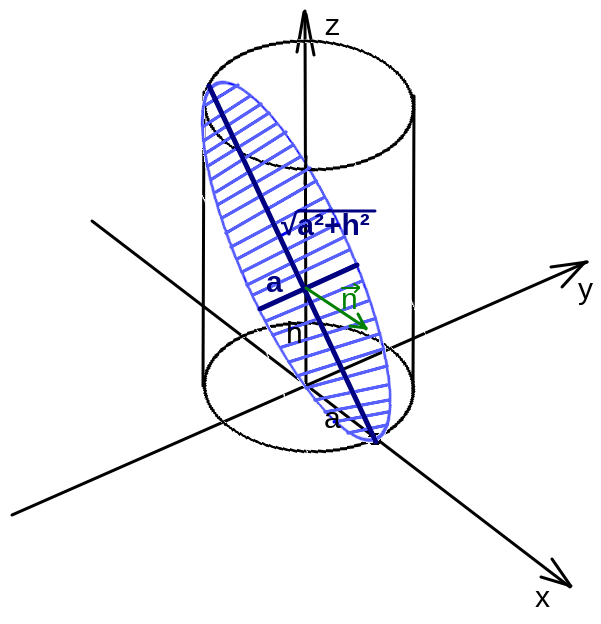
\includegraphics[scale=0.75]{lec25-cylinder}
			\end{center}
			
			Получаем фигуру, которая является сечением цилиндра плоскостью.
			
			Плоскость: 
			\[x = 0 \implies z = a,\]
			\[z = 0 \implies x = h.\]
			
			Сечением будет эллипс с полуосями $a$ и $\sqrt{a^2 + h^2}$. Воспользуемся 
			формулой Стокса и в качестве поверхности $\pi$ возьмем плоскость с вектором 
			нормали
			\[ \vec{N}\left( \frac{1}{a}, 0 , \frac{1}{h} \right). \]
			Его длина:
			\[ \left| \vec{N} \right|= \sqrt{\frac{1}{a^2} + \frac{1}{h^2} } = 
			\frac{\sqrt{a^2 + h^2}}{ah}.  \]
			Его направляющие косинусы:
			\[ \vec{n} = \left( \frac{h}{\sqrt{a^2 + h^2}}, 0, \frac{a}{\sqrt{a^2 + 
			h^2}} \right). \]
			
			Если смотреть с положительной стороны $Oz$, движение будет направлено 
			против часовой стрелки, т.~е. согласовано.
			Тогда по формуле Стокса:
			\[ I = \iint \limits_{\pi} -2 \, dxdy -2 \, dydz -2 \, dzdx = \left[ 
			\text{перейдем от ПовИ-2 к ПовИ-1} \right] =  \]
			\[ = -2 \iint \limits_{\pi} \left(\frac{h}{\sqrt{a^2 + h^2}} +  0 + 
			\frac{a}{\sqrt{a^2 + h^2}}\right) \, ds = -2 \iint \limits_{\pi} 
			\frac{h+a}{\sqrt{a^2 + h^2}}  \, ds = -2\frac{a+h}{\sqrt{a^2 + h^2}}  
			S_{\text{эллипса}} = \]
			\[ = -2\frac{a+h}{\sqrt{a^2 + h^2}} \pi a \sqrt{a^2 + h^2} = -2 \pi a 
			\left( a+h \right).       \]
		\end{example}
			
		\section{Основная Теорема о КрИ в пространстве}
		
		Говорят, что область $D \subset \R ^3$	\emph{поверхностно односвязная}, если 
		на любой замкнутый контур $l \subset D$ можно натянуть поверхность, лежащую 
		в $D$.
		
		\begin{theorem}
			Пусть в поверхностно односвязной области $D$ заданы функции $P,Q,R$~--- 
			непрерывные и имеющие частные производные первого порядка. Следующие 
			условия равносильны:
			
			\begin{enumerate}[label=\arabic*\,$^{\circ}$]
				\item $\displaystyle\forall L \subset D \quad \oint \limits_L P \, dx + Q 
				\, dy + R \, dz = 0.$
				\item $\displaystyle\int \limits_{{\tiny \overbow{AB}}} P \, dx   + Q \, 
				dy + R \, dz \,$ не зависит от пути интегрирования.
				\item Выражение $P\,dx + Q\,dy+R\,dz$ является полным дифференциалом, 
				т.~е. 
				\[ \exists F : dF = P\,dx + Q\,dy+R\,dz. \]
				\item В $D$ выполнены \emph{условия Эйлера}:
				\[ Q_x' = P_y', \quad Q_z' = R_y', \quad P_z' = R_x'. \]
			\end{enumerate}
		\begin{proof}
			Доказательство проводится по той же схеме, что и доказательство аналогичной 
			теоремы для КрИ на плоскости.
		\end{proof}	
			
		\end{theorem}
		
		Функция $F = F\left( x,y,z\right) $ может быть найдена, например, по формуле 
		ниже (в некоторых простейших случаях):
		
		\[ F\left( x,y,z\right) = \int_{x_0}^{x} P\left(x,y,z \right)dx + 
		\int_{y_0}^{y} Q\left(x_0,y,z \right)dy + \int_{z_0}^{z} R\left(x_0,y_0,z 
		\right)dz, \]
		где $\left( x_0,y_0,z_0\right) $~--- произвольная фиксированная точка в 
		области $D$.
	\end{document}
